\documentclass[11pt]{article}

\usepackage{comment} % enables the use of multi-line comments (\ifx \fi) 
\usepackage[a4paper,margin=1cm]{geometry}
\usepackage[utf8]{inputenc}
\usepackage[ngerman]{isodate}
\usepackage{gensymb}
\usepackage{graphicx}
\usepackage{booktabs}% http://ctan.org/pkg/booktabs
\usepackage{tabularx}
\usepackage{ltablex} % Longtables with tabularx
\usepackage[x11names]{xcolor}
\usepackage{amsmath}
\usepackage{amssymb}
\usepackage{array}
\usepackage{wrapfig}
\usepackage{subcaption}
\usepackage{lscape}
\usepackage{geometry}
\usepackage{multicol}
\usepackage{bm}
\usepackage{enumitem}
\usepackage{mdframed}
\usepackage{scalerel}
\usepackage{stackengine}
\usepackage{mathtools}
\usepackage{pdfpages}

% Code highlighting
\usepackage{minted}
\surroundwithmdframed{minted}

% Be able to caption equations and float them in place
\usepackage{float}

\usepackage{csquotes}
\usepackage{hyperref}

\newmdtheoremenv{theorem}{Theorem}
\geometry{a4paper, margin=2.4cm}

\newcommand\equalhat{\mathrel{\stackon[1.5pt]{=}{\stretchto{\scalerel*[\widthof{=}]{\wedge}{\rule{1ex}{3ex}}}{0.5ex}}}}
\newcommand\defeq{\mathrel{\overset{\makebox[0pt]{\mbox{\normalfont\tiny def}}}{=}}}
\newcolumntype{C}{>{\centering\arraybackslash}X}

\DeclarePairedDelimiter\abs{\lvert}{\rvert}
\DeclarePairedDelimiter\norm{\lVert}{\rVert}

\setcounter{tocdepth}{3}
\setcounter{secnumdepth}{3}

\graphicspath{{./img/}}

\begin{document}
	
\title{Machine Learning in Computer Vision FS20}
\author{Pascal Baumann\\pascal.baumann@stud.hslu.ch}
\maketitle



For errors or improvement raise an issue or make a pull request on the \href{https://github.com/KilnOfTheSecondFlame/mse_summaries}{github repository}.

\tableofcontents
\newpage


\section{Image Handling in Python}

\begin{minted}{python}
plt.imshow(np.hstack((im_float, im_float)), cmap="gray", vmin=0, vmax=1);
\end{minted}

\begin{center}
	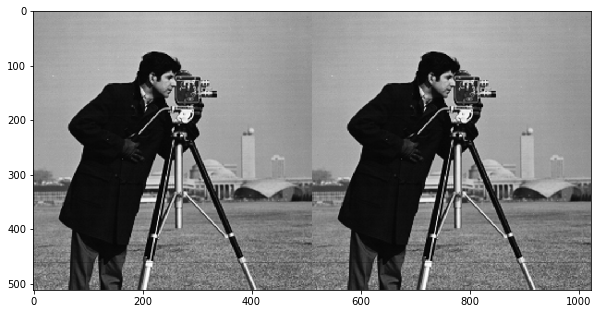
\includegraphics[width=0.7\linewidth]{img/hstack_image}
\end{center}

\subsection{Fading an Image}

\begin{minted}{python}
im = skimage.io.imread("data/snoopy.png")
im = im/255 # tip: use floating point values

ims = []

im_temp = np.fliplr(im)
ims.append(im_temp)
for i in range(1,5):
	im_temp = im_temp + (0.4)**i
	ims.append(im_temp)

plt.imshow(np.hstack(ims),vmin=0, vmax=1, cmap="gray")
\end{minted}

\begin{center}
	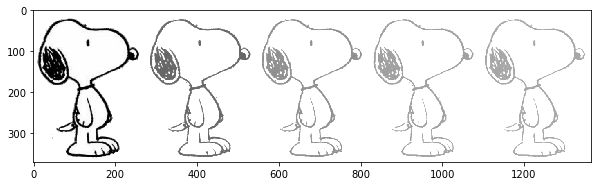
\includegraphics[width=0.7\linewidth]{img/snoopy_fade}
\end{center}

\subsubsection{IPyWidgets}
\begin{minted}{python}
@interact(thresh=widgets.FloatSlider(min=0.0, max=0.5, step=0.01, value=0.2))
def threshold(thresh):
	im_thresh = []
	for line in im:
		im_thresh.append([pixel if pixel > np.min(line) + thresh else float(0) for pixel in line])
	plt.imshow(im_thresh, cmap="gray", vmin=0, vmax=1)
	plt.show()
\end{minted}

\begin{center}
	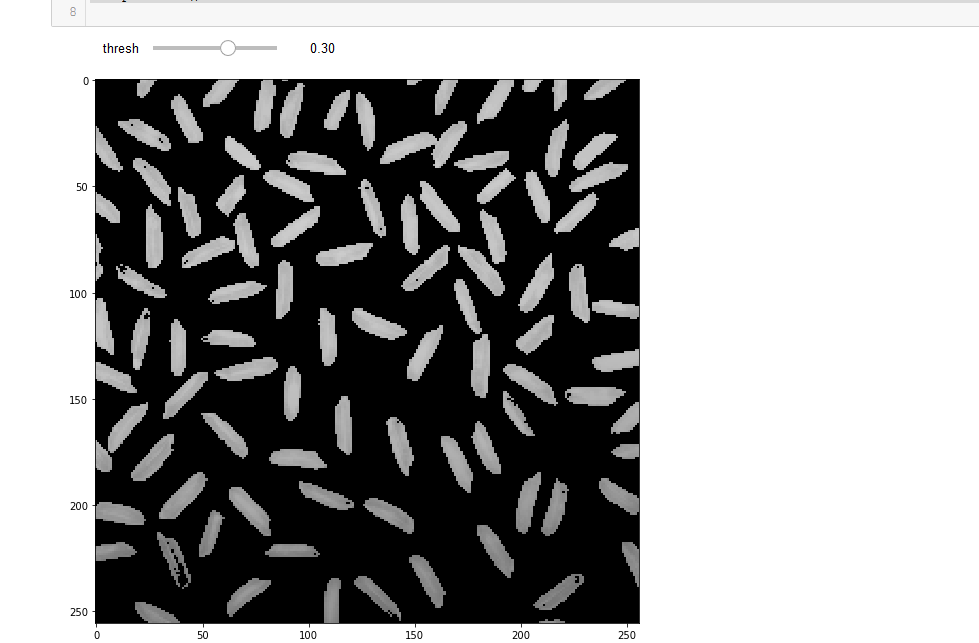
\includegraphics[width=0.6\linewidth]{img/ipywidgets_example}
\end{center}

\section{Local Filtering and Edge Detection}
\subsection{Filtering}
The naive approach of local filtering is taking just a moving average of the pixels in the neighbourhood.

\subsection{Edge Detection}
Although intuitive for humans to detect, edge detection was a hard problem in image processing. And edge is defined by a rapid change in the intensity, which can be exploited by calculating the derivative.

\begin{center}
	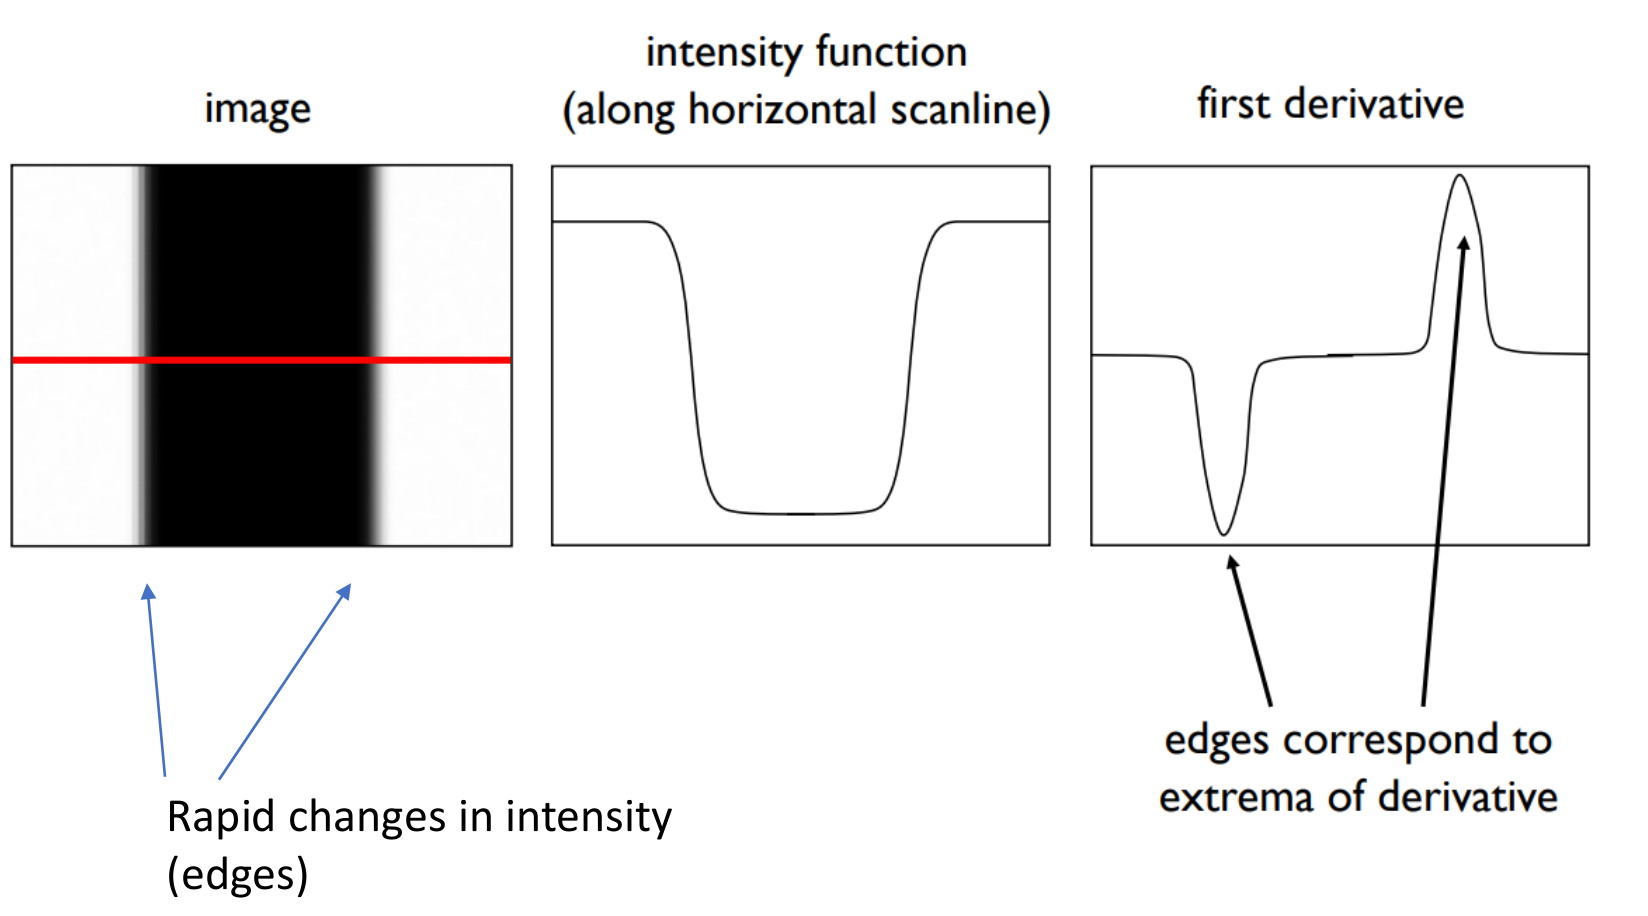
\includegraphics[width=0.6\linewidth]{img/1D_edge_derivative}
\end{center}

\noindent
In two dimensions the derivative corresponds to the gradient $\nabla f = \left[\frac{\partial f}{\partial x},\frac{\partial f}{\partial y}\right]$, which points from the edge towards the increase in intensity or the lighter side.

\begin{align}
\shortintertext{Gradient}
\nabla f &= \left[ \frac{\partial f}{\partial x}, \frac{\partial f}{\partial y} \right]
\shortintertext{Gradient Direction}
\theta &= \tan^{-1} \left( \frac{\partial f}{\partial x} / \frac{\partial f}{\partial y} \right)
\shortintertext{Gradient Magnitude (strength of the edge)}
\norm{\nabla f} &= \sqrt{\left(\frac{\partial f}{\partial x}\right)^2 + \left(\frac{\partial f}{\partial y} \right)^2 }
\end{align}

But not all important edges have strong gradients, nor are all strong gradients important edges.

\subsubsection{Computing the Gradient on an Image}

Approximate Gradient in direction of $ \frac{\partial f}{\partial x} $: Convolution with kernel \begin{tabular}{|c|c|}
	\hline
	-1 & 1\\
	\hline
\end{tabular}

\noindent
Approximate Gradient in direction of $ \frac{\partial f}{\partial y} $: Convolution with kernel \begin{tabular}{|c|}
	\hline
	-1 \\
	\hline
	1\\
	\hline
\end{tabular}

The drawback of the gradient is, that it is very sensitive to noise:
\begin{figure}[H]
	\centering
	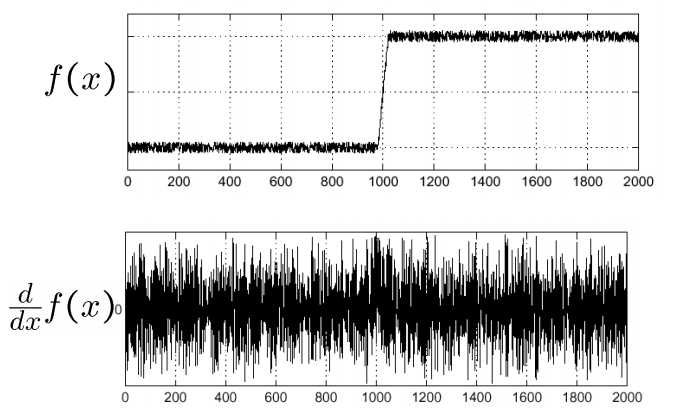
\includegraphics[width=0.7\linewidth]{img/noise_gradient}
	\caption{Gradient of a 1D function, where it is clear how it amplifies noise and may conceal a weak signal}
	\label{fig:noisegradient}
\end{figure}

\noindent
The solution to this is, to first smooth the function and then apply the gradient.

The larger the value of $\sigma$ the more smoothing is applied and different kind of features can be identified.
\begin{itemize}[leftmargin=*, labelindent=3.5cm, labelsep=0.5cm]
	\item[\textbf{large value of $\sigma$}] larger scale or stronger edges detected
	\item[\textbf{smaller value of $\sigma$}] finer details detected
\end{itemize}

\noindent
\begin{minipage}{0.6\textwidth}
	In practice a convolution with a derivative of Gaussian filter is calculated to compute the gradients.
	
	This is equivalent to smoothing with a Gaussian and then taking the derivative.
\end{minipage}
\begin{minipage}{0.4\textwidth}
	\begin{center}
		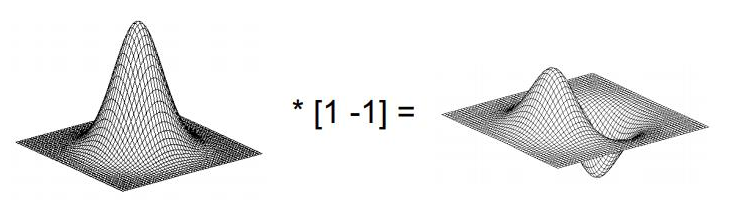
\includegraphics[width=0.6\linewidth]{img/derivative_gaussian_filter}
	\end{center}
\end{minipage}

\begin{figure}[H]
	\centering
	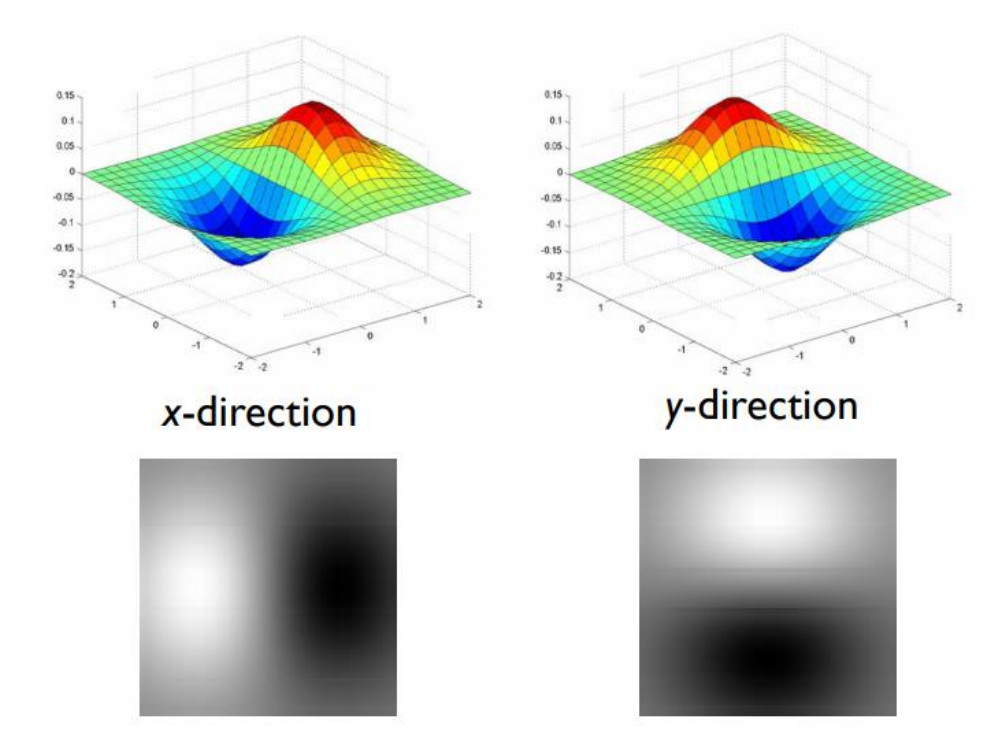
\includegraphics[width=0.6\linewidth]{img/derivative_gaussian_filter2}
	\caption{Derivative of Gaussian Filters}
	\label{fig:derivativegaussianfilter2}
\end{figure}

\begin{itemize}
	\item A Gaussian smoothing filter removes high-frequency components
	\item Values of a Gaussian smoothing filter sum to one
	\item Derivative filters contain some negative value and values sum to zero
	\item Derivative filters yield large responses at points with high contrast
\end{itemize}

% TODO Canny Edge Detection

% TODO Hysteresis Thresholding



\end{document}
